\section{PDCA o Ciclo di Deming}
Ogni processo deve essere organizzato basandosi sul principio del miglioramento
continuo (o ciclo di Deming\pedice):

~\newline\textbf{Plan (Pianificare):} viene definito un piano che basandosi sulla definizione di
problemi e obiettivi pianifica compiti, assegna responsabilità, studia il caso,
analizza le cause della criticità e definisce azioni correttive;

~\newline\textbf{Do (Eseguire):} vengono implementate le attività secondo le linee definite durante
la fase Plan;

~\newline\textbf{Check (Valutare):} viene verificato l’esito delle azioni di miglioramento rispetto
alle attese;

~\newline\textbf{Act (Agire):} vengono applicate le correzioni necessarie per colmare le carenze
rilevate e vengono standardizzate le attività correttamente eseguite.

\begin{figure}[!htbp]
	\centering
	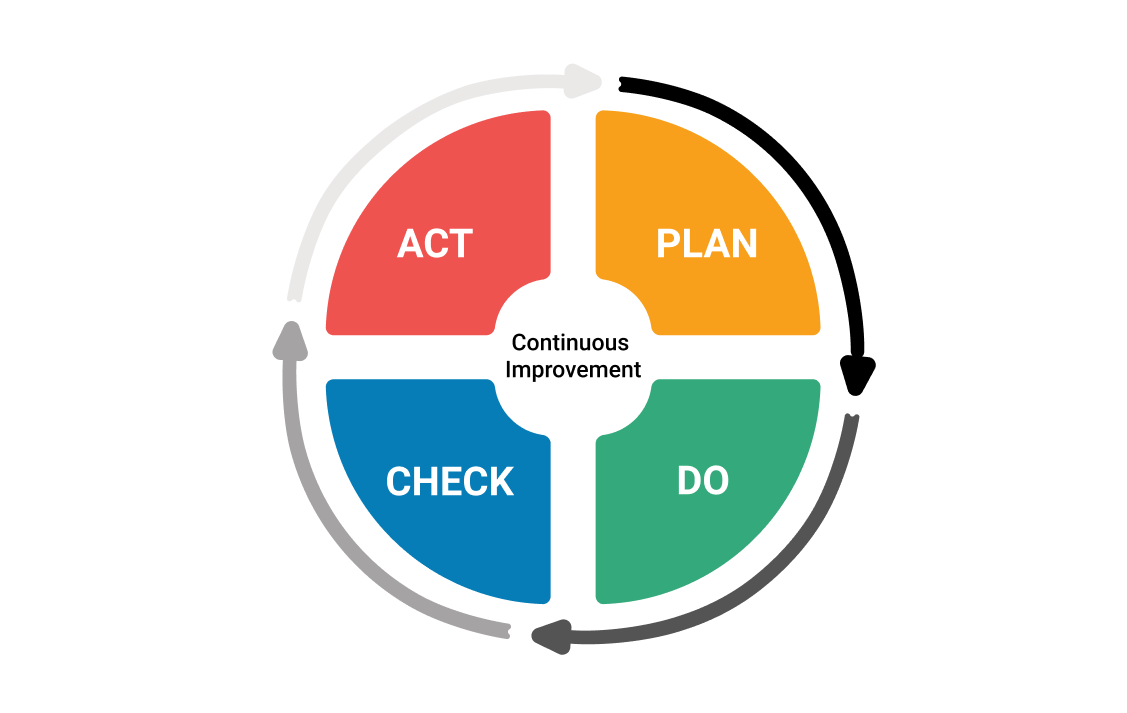
\includegraphics[scale=0.3]{pdca.png}
	\caption{Ciclo di Deming}
\end{figure}